\documentclass[aspectratio=169]{beamer}
\usepackage[utf8]{luainputenc}
\usepackage[TS1,T1]{fontenc}
\usepackage{babel}
\usetheme[pagenum,navbar,ddc]{tud}
\usepackage{xcolor}
\usepackage{listings}
\usepackage{tikz}
\usepackage{caption}
\usepackage{subcaption}
\usepackage{hyperref}
\usepackage{wrapfig}
\usepackage{float}

\hypersetup{
    colorlinks=false,
    linkcolor=black,
    filecolor=magenta,      
    urlcolor=black,
}

\definecolor{mygreen}{rgb}{0,0.6,0}
\definecolor{mygray}{rgb}{0.5,0.5,0.5}
\definecolor{mymauve}{rgb}{0.58,0,0.82}

\lstset{ 
  backgroundcolor=\color{white},   % choose the background color; you must add \usepackage{color} or \usepackage{xcolor}; should come as last argument
  basicstyle=\footnotesize\ttfamily,        % the size of the fonts that are used for the code
  breakatwhitespace=false,         % sets if automatic breaks should only happen at whitespace
  breaklines=true,                 % sets automatic line breaking
  captionpos=n,                    % sets the caption-position to bottom
  commentstyle=\color{mygreen},    % comment style
  deletekeywords={...},            % if you want to delete keywords from the given language
  escapeinside={\%*}{*)},          % if you want to add LaTeX within your code
  extendedchars=true,              % lets you use non-ASCII characters; for 8-bits encodings only, does not work with UTF-8
  firstnumber=0,                % start line enumeration with line 1000
  frame=single,	                   % adds a frame around the code
  keepspaces=true,                 % keeps spaces in text, useful for keeping indentation of code (possibly needs columns=flexible)
  keywordstyle=\color{blue},       % keyword style
  language=Octave,                 % the language of the code
  morekeywords={*,...},            % if you want to add more keywords to the set
  numbers=left,                    % where to put the line-numbers; possible values are (none, left, right)
  numbersep=5pt,                   % how far the line-numbers are from the code
  numberstyle=\tiny\color{mygray}, % the style that is used for the line-numbers
  rulecolor=\color{black},         % if not set, the frame-color may be changed on line-breaks within not-black text (e.g. comments (green here))
  showspaces=false,                % show spaces everywhere adding particular underscores; it overrides 'showstringspaces'
  showstringspaces=false,          % underline spaces within strings only
  showtabs=false,                  % show tabs within strings adding particular underscores
  stepnumber=2,                    % the step between two line-numbers. If it's 1, each line will be numbered
  stringstyle=\color{mymauve},     % string literal style
  tabsize=2,	                   % sets default tabsize to 2 spaces
  title=\lstname                   % show the filename of files included with \lstinputlisting; also try caption instead of title
}

\title[System Monitoring via Hardware Performance Counter and TEE Design]{System Monitoring via Hardware Performance Counter and TEE Design}
\author{Pascal Scholz}
\einrichtung{Dresden University of Technology}
\institut{Institute of Systems Architecture}
\professur{Chair of Operating Systems}
\einrichtung{}
\date{November 8th, 2024}

\newcommand*\inmm[1]{\pgfmathsetmacro\inmmwert{#1 / 1mm}\inmmwert}
\makeatletter
\newcommand*\inpt[1]{\setlength\@tempdima{#1}\the\@tempdima}
\makeatother

\AtBeginSection[]{\partpage{\usebeamertemplate***{part page}}}
\begin{document}

\maketitle

\mode<presentation>{\setbeamertemplate{page number in footline}[frame number]}

%-----------------------------------------------------------------------------------------------------------------------
\begin{frame}{Motivation}
    \begin{figure}
        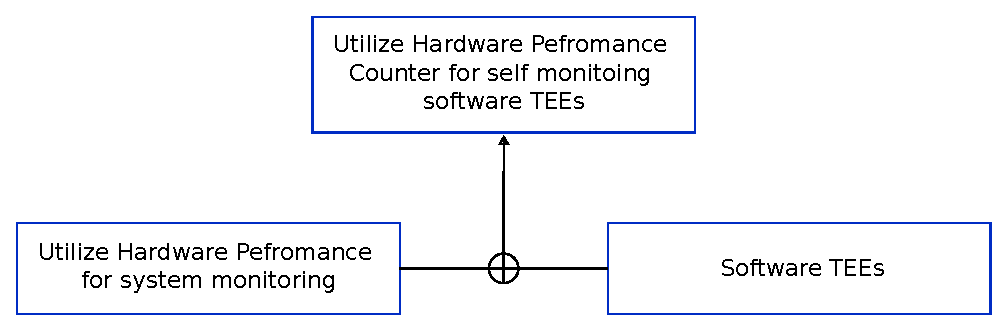
\includegraphics[width=\textwidth]{images/components.eps}
    \end{figure}
\end{frame}
%-----------------------------------------------------------------------------------------------------------------------
\begin{frame}{Hardware Performance Counters}
    \begin{itemize}
        \item Events are either architectural (fixed) or non-architectural (PMU)
        \item Different amount of counters for non-/architectural events
        \item Each programming MSR has a corresponding counter MSR
        \item Either polling or performance-measurement-interrupt (PMI)
    \end{itemize}
\end{frame}
%-----------------------------------------------------------------------------------------------------------------------
\begin{frame}{Trusted Execution Environments}
    \textit{An execution environment that runs alongside but isolated from an REE (regular execution environment).
        A TEE has security capabilities and meets certain security-related
        requirements} \\ - GlobalPlatform Specification
    \bigskip
    \begin{itemize}
        \item protects assets from general software attacks
        \item defines rigid safeguards as to data and functions
        \item resists a set of defined threats
    \end{itemize}
\end{frame}

%-----------------------------------------------------------------------------------------------------------------------
\begin{frame}{Hardware Performance Counters for System Reliability - Overview}
    \begin{itemize}
        \item Evaluates system reliability by monitoring Performance counters
        \item Theory: System anomalies are reflected by abnormal software behavior
              \\ $\rightarrow$ Software anomalies are visible through Performance Counters
        \item Uses Gem5 simulator to simulate single stuck fault
        \item Events measured:
              \begin{enumerate}
                  \item Instructions committed
                  \item Number of function calls
                  \item Number of integer instructions
                  \item Number of load instructions
              \end{enumerate}
        \item Sampling of Performance Counters every 10ms
    \end{itemize}
\end{frame}
%-----------------------------------------------------------------------------------------------------------------------
\begin{frame}{Hardware Performance Counters for System Reliability - Findings}
    \begin{itemize}
        \item Fault injection leads to exceptions (e.g. Page fault, invalid OpCode ...)
        \item Abnormal program behavior/recovering from exception was reflected in PC
        \item With timing data from sampling, authors were able to recover from faults
        \item Without timing data, one can only tell if program terminated early
              \begin{itemize}
                  \item Cannot differentiate between crash and termination with error
              \end{itemize}
    \end{itemize}
\end{frame}
%-----------------------------------------------------------------------------------------------------------------------
\begin{frame}{Malicious Firmware Detection with Hardware Performance Counters - Overview}
    \begin{itemize}
        \item Embedded device: ROM contains bootloader, that loads Firmware/OS
        \item Firmware/OS then loads application
        \item Goal: Monitor control flow integrity (CFI) for detecting malicious modification
        \item ConFirm monitor CFI through reading Performance Counters
        \item ConFirm embedded into bootloader to protect it against manipulation
    \end{itemize}
\end{frame}
%-----------------------------------------------------------------------------------------------------------------------
\begin{frame}{Malicious Firmware Detection with Hardware Performance Counters - Details}
    \begin{itemize}
        \item ConFirm consists of three modules:
              \begin{enumerate}
                  \item Insertion module, that replaces instructions with checkpoints
                  \item Driver for reading and managing performance counters
                  \item Database storing valid PC signatures
              \end{enumerate}
        \item PC signatures are collected running the firmware
    \end{itemize}
\end{frame}
%-----------------------------------------------------------------------------------------------------------------------
\begin{frame}{Malicious Firmware Detection with Hardware Performance Counters - Findings}
    \begin{itemize}
        \item HPC measurements need to be reliable and reproducible
        \item On average HPC measurements showed are derivation of 18.9\% (ARM) and 16.7\% (PowerPC)
        \item Signature based approach performs good for firmware with simple control flow
        \item Bad performance for complex control flow
              \\$\rightarrow$ ML approach used to improve results
        \item To reduce system load, ML-approach was run remote
    \end{itemize}
\end{frame}

%-----------------------------------------------------------------------------------------------------------------------
\begin{frame}{CFIMon: Detecting Violation of Control Flow Integrity using Performance Counters - Overview}
    \begin{itemize}
        \item Idea: Control flow monitoring through performance counters
        \item AMD manuel states that IP in interrupt based sampling differs up to 72 instructions
              \\ $\rightarrow$ Use Intel Precise Event Based Sampling (PEBS) and AMD Instruction-based sampling (IBS)
        \item Branch Trace Store (BTS) records all control flow events
              \\ $\rightarrow$ Enables monitoring of whole application control flow
        \item Analyze legal Control flow in an offline phase, Monitor in an online phase
    \end{itemize}
\end{frame}
%-----------------------------------------------------------------------------------------------------------------------
\begin{frame}{CFIMon: Detecting Violation of Control Flow Integrity using Performance Counters - Details}
    \begin{itemize}
        \item Static analysis yields set of allowed addresses for direct jumps
        \item Run time analysis yields addresses for indirect jumps
              \\ $\rightarrow$ Set of legal jump addresses is created
        \item On run time: Divide branches taken into legal, suspicious and illegal
              \\ $\rightarrow$ Illegal branching triggers a defined response
              \\ $\rightarrow$ If the number of suspicious branches exceeds threshold, the control flow is considered illegal
    \end{itemize}
\end{frame}
%-----------------------------------------------------------------------------------------------------------------------
\begin{frame}{CFIMon: Detecting Violation of Control Flow Integrity using Performance Counters - Findings}
    \begin{itemize}
        \item All control flow exploits tested could be identified
        \item Performance overhead for analysis is 6.1\%
        \item No false positives when using the PoC implementation in daily use over multiple days
    \end{itemize}
\end{frame}
%-----------------------------------------------------------------------------------------------------------------------
\begin{frame}{Detecting Spectre Attacks Using Hardware Performance Counters - Basics}
    \begin{itemize}
        \item Two variants of Spectre attacks:
              \begin{enumerate}
                  \item Variant one: Exploits conditional branch prediction
                  \item Variant two: Exploits unconditional jump target prediction
              \end{enumerate}
        \item Training of branch predictor through executing the same path multiple times
              \\ $\rightarrow$ mispredictions drop below expected amount
        \item Attack itself relies on timing and therefore executes cache flushes
              \\ $\rightarrow$ Number of Cache flushes and cache misses rise
    \end{itemize}
\end{frame}
%-----------------------------------------------------------------------------------------------------------------------
\begin{frame}{Detecting Spectre Attacks Using Hardware Performance Counters - Detection}
    \begin{itemize}
        \item Microarchitectural effects observable through hardware counters
        \item Monitored events
              \begin{enumerate}
                  \item Cache references
                  \item Cache misses
                  \item Branch instructions retired
                  \item Branch mispredictions
              \end{enumerate}
        \item Sliding windows for PC sampling
        \item Training of different ML algorithms
    \end{itemize}
\end{frame}
%-----------------------------------------------------------------------------------------------------------------------
\begin{frame}{Detecting Spectre Attacks Using Hardware Performance Counters - Findings}
    \begin{itemize}
        \item Default attack can be reliably detected
        \item Reducing the attacks speed (and bandwidth) makes detection less reliable
        \item Splitting attack up into atomically executed parts increases attack success rate
        \item This also allows to insert obfuscation code to be inserted
        \item Obfuscation reduces detection rate
        \item Multi layer perceptron network can still reliably detect attack
    \end{itemize}
\end{frame}
%-----------------------------------------------------------------------------------------------------------------------
\begin{frame}{Towards Self-monitoring Enclaves: Side-Channel Detection Using Performance Counters - Overwiev}
    \begin{itemize}
        \item Studies Load Value injection attacks (LVI)
        \item Authors identify Cache side channels as a high risk attack vector
        \item Thesis: LVI attacks lead to abnormal program behavior
              \\ $\rightarrow$ Effects on hardware should be observable
        \item Monitor performance counters to detect attacks
    \end{itemize}
\end{frame}
%-----------------------------------------------------------------------------------------------------------------------
\begin{frame}{Towards Self-monitoring Enclaves: Side-Channel Detection Using Performance Counters - Concept}
    \begin{itemize}
        \item LVI attacks induce high count of page faults
        \item Moreover LVI attacks produce a abnormal high count of cache misses and cache references
        \item Events measures:
              \begin{enumerate}
                  \item Total number of instructions
                  \item LLC misses
                  \item LLC references
                  \item Page faults (minor, major, total)
              \end{enumerate}
    \end{itemize}
\end{frame}
%-----------------------------------------------------------------------------------------------------------------------
\begin{frame}{Towards Self-monitoring Enclaves: Side-Channel Detection Using Performance Counters - Findings}
    \begin{itemize}
        \item LVI were detected using a simple threshold mechanism
              \begin{itemize}
                  \item L1D cache injection was harder to detect
              \end{itemize}
        \item Authors assume ML could help improving the results
        \item Authors conclude that SGX could benefit form self monitoring
    \end{itemize}
\end{frame}
%-----------------------------------------------------------------------------------------------------------------------
\begin{frame}{Isolating Program Execution on L4Re/Fiasco - Overview}
    \begin{itemize}
        \item Diplomarbeit of Hanna Reitz in cooperation with Kernkonzept
        \item Goal: Creating isolated enclaves within L4Re
        \item Software based solution, leverage isolation properties if L4Re
        \item Assumes Fiasco is trustworthy
        \item TPM is hardware root of trust
    \end{itemize}
\end{frame}
%-----------------------------------------------------------------------------------------------------------------------
\begin{frame}{Isolating Program Execution on L4Re/Fiasco - Components}
    \begin{itemize}
        \item Enma (Enclave Manager) manages and creates Enclaves
        \item TCB: Hardware + Firmware + Bootloader + Fiasco.OC + sigma0 + moe + Enma
        \item TPM verifies that software stack is unmodified
        \item Quoting enclave verifies state of other enclaves through Remote Attestation
        \item Works without SGX or other hardware features
    \end{itemize}
\end{frame}
%-----------------------------------------------------------------------------------------------------------------------
\begin{frame}{OpenVMM \& OpenHCL}
    \begin{itemize}
        \item Microsofts VMM with OpenHCL being the underlying Paravisor
              \begin{itemize}
                  \item Paravisor: Cooperates with Guest for increased performance
              \end{itemize}
        \item Written in Rust
        \item Developed closed source since 2019, open source since October 2024
    \end{itemize}
\end{frame}
%-----------------------------------------------------------------------------------------------------------------------
\begin{frame}{OpenHCL in detail}
    \begin{itemize}
        \item Host so called partitions (VMs)
        \item Backed either by hardware features or Virtual Secure Mode (VSM)
        \item Utilizes SLAT for address space isolation
        \item Manages vCPUs and other resources
    \end{itemize}
\end{frame}
%-----------------------------------------------------------------------------------------------------------------------
\begin{frame}{Virtual Secure Mode (VSM)}
    \begin{itemize}
        \item Offers interface to enable creation and modification of partitions
        \item Assigns each partition a Virtual Trust Level (VTL)
        \item Lower VTL can't interact with higher VTL
        \item OpenHCL runs in VTL2, secure Kernel in VTL1,
    \end{itemize}
\end{frame}
%-----------------------------------------------------------------------------------------------------------------------
% \begin{frame}{Some graphics}
%     \begin{figure}
%         \begin{subfigure}[]{0.45\textwidth}
%             \includegraphics[width=\textwidth]{images/example.png}
%             \caption{Smiling example face}
%         \end{subfigure}
%         \begin{subfigure}[]{0.45\textwidth}
%             \includegraphics[width=\textwidth]{images/example.png}
%             \caption{Teh same smile again}
%         \end{subfigure}
%     \end{figure}
% \end{frame}
%-----------------------------------------------------------------------------------------------------------------------
\end{document}
